\documentclass[14pt,a4paper]{article}
\usepackage[a4paper, mag=1000, left=2cm, right=2cm, top=2cm, bottom=2cm, headsep=0.7cm, footskip=cm]{geometry}
\usepackage[utf8x]{inputenc}
\usepackage[T1,T2A]{fontenc}
\usepackage[english,russian]{babel}
\usepackage{indentfirst}
\usepackage[dvipsnames]{xcolor}
\usepackage[colorlinks]{hyperref}
\usepackage{listings} 
\usepackage{fancyhdr}
\usepackage{caption}
\usepackage{subfig}
\usepackage{color}
\usepackage{here}
\usepackage{array}
\usepackage{multirow}
\usepackage{subcaption}
\usepackage{amsmath}
\usepackage{latexsym}
\usepackage{graphicx}
\hypersetup{
	colorlinks = true,
	linkcolor  = black
}

\DeclareCaptionFont{white}{\color{white}} 

\sloppy

% Listing description

\usepackage{listings}
\usepackage{caption}
\DeclareCaptionFont{white}{\color{white}}
\DeclareCaptionFormat{listing}{\colorbox{gray}{\parbox{\dimexpr\textwidth-1.72\fboxsep\relax}{#1#2#3}}}
\captionsetup[lstlisting]{format=listing,labelfont=white,textfont=white,margin=0pt}
\lstset{language=C,
	basicstyle=\footnotesize,
	keepspaces=true,
	tabsize=4,               
	frame=single,                           % Single frame around code
	rulecolor=\color{black},
	captionpos=b,
	showstringspaces=false,	
	abovecaptionskip=-0.9pt,
	xleftmargin=3.4pt,
	xrightmargin=2.6pt,
	breaklines=true,
	postbreak=\raisebox{0ex}[0ex][0ex]{\ensuremath{\color{black}\hookrightarrow\space}},
	xleftmargin=3.2pt,
	literate={а}{{\selectfont\char224}}1
	{~}{{\textasciitilde}}1
	{б}{{\selectfont\char225}}1
	{в}{{\selectfont\char226}}1
	{г}{{\selectfont\char227}}1
	{д}{{\selectfont\char228}}1
	{е}{{\selectfont\char229}}1
	{ё}{{\"e}}1
	{ж}{{\selectfont\char230}}1
	{з}{{\selectfont\char231}}1
	{и}{{\selectfont\char232}}1
	{й}{{\selectfont\char233}}1
	{к}{{\selectfont\char234}}1
	{л}{{\selectfont\char235}}1
	{м}{{\selectfont\char236}}1
	{н}{{\selectfont\char237}}1
	{о}{{\selectfont\char238}}1
	{п}{{\selectfont\char239}}1
	{р}{{\selectfont\char240}}1
	{с}{{\selectfont\char241}}1
	{т}{{\selectfont\char242}}1
	{у}{{\selectfont\char243}}1
	{ф}{{\selectfont\char244}}1
	{х}{{\selectfont\char245}}1
	{ц}{{\selectfont\char246}}1
	{ч}{{\selectfont\char247}}1
	{ш}{{\selectfont\char248}}1
	{щ}{{\selectfont\char249}}1
	{ъ}{{\selectfont\char250}}1
	{ы}{{\selectfont\char251}}1
	{ь}{{\selectfont\char252}}1
	{э}{{\selectfont\char253}}1
	{ю}{{\selectfont\char254}}1
	{я}{{\selectfont\char255}}1
	{А}{{\selectfont\char192}}1
	{Б}{{\selectfont\char193}}1
	{В}{{\selectfont\char194}}1
	{Г}{{\selectfont\char195}}1
	{Д}{{\selectfont\char196}}1
	{Е}{{\selectfont\char197}}1
	{Ё}{{\"E}}1
	{Ж}{{\selectfont\char198}}1
	{З}{{\selectfont\char199}}1
	{И}{{\selectfont\char200}}1
	{Й}{{\selectfont\char201}}1
	{К}{{\selectfont\char202}}1
	{Л}{{\selectfont\char203}}1
	{М}{{\selectfont\char204}}1
	{Н}{{\selectfont\char205}}1
	{О}{{\selectfont\char206}}1
	{П}{{\selectfont\char207}}1
	{Р}{{\selectfont\char208}}1
	{С}{{\selectfont\char209}}1
	{Т}{{\selectfont\char210}}1
	{У}{{\selectfont\char211}}1
	{Ф}{{\selectfont\char212}}1
	{Х}{{\selectfont\char213}}1
	{Ц}{{\selectfont\char214}}1
	{Ч}{{\selectfont\char215}}1
	{Ш}{{\selectfont\char216}}1
	{Щ}{{\selectfont\char217}}1
	{Ъ}{{\selectfont\char218}}1
	{Ы}{{\selectfont\char219}}1
	{Ь}{{\selectfont\char220}}1
	{Э}{{\selectfont\char221}}1
	{Ю}{{\selectfont\char222}}1
	{Я}{{\selectfont\char223}}1,
	extendedchars=true
}

\DeclareCaptionFormat{hfillstart}{\hfill#1#2#3\par}
\captionsetup[table]{format=hfillstart,labelsep=newline,justification=centering,skip=-10pt,textfont=bf}


\usepackage{float}

\begin{document}

\begin{titlepage}
    \centering
    \textsc{Санкт-Петербургский политехнический университет Петра Великого}\\[3mm]
    \textsc{Институт компьютерных наук и технологий}\\[3mm]
    \textsc{Кафедра компьютерных систем и программных технологий}
	
	\vfill
	
	\textbf{Отчёт по лабораторной работе }\\[3mm]
	по курсу «Проектирование ОС и компонентов»\\[3mm]
	по теме «Драйвер символьного устройства»\\[41mm]
	
    \begin{flushright}
	\begin{minipage}{.35\textwidth}
		Выполнил студент гр. 13541/2:\\
		Волкова М. Д.\\[3mm]
		Проверил преподаватель:\\
		Душутина Е. В.
	\end{minipage}
    \end{flushright}
	
	\vfill

	Санкт-Петербург\\
	\the\year\ г.
\end{titlepage}


\renewcommand\contentsname{\centerline{Содержание}}
\tableofcontents
\newpage


\section{Цель работы}
\par Необходимо написать драйвер для flash устройства с произвольной функциональностью. Драйвер может работать как в пространстве пользователя, так и в пространстве ядра. Целевая операционная система Windows.

\subsection{Характеристики системы}
\begin{figure}[H]
  \centering
  \fbox{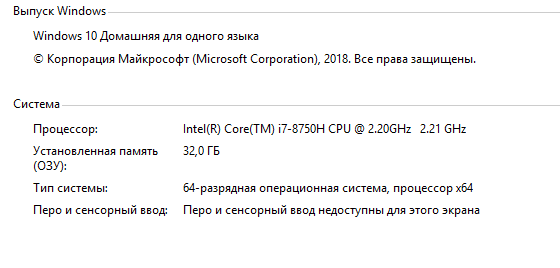
\includegraphics[width = \textwidth]{images/system.png}}
  \caption{Система}
\end{figure}

\section{Общее описание}

\par Flash накопитель - запоминающее устройство, использующее в качестве носителя флеш-память, и подключаемое к компьютеру или иному считывающему устройству по интерфейсу USB.\\

\par Поэтому разработка драйвера для flash накопителя является разработкой драйвера USB устройства.
Универсальная последовательная шина (USB) обеспечивает расширяемый последовательный интерфейс Plug and Play с возможностью «горячей» замены, который обеспечивает подключение для периферийных устройств, таких как клавиатуры, мыши, принтеры, сканеры, устройства хранения и т.д.\\

\par Драйвер USB-клиента - это программное обеспечение, установленное на компьютере, которое обменивается данными с оборудованием для обеспечения работы устройства. Если устройство принадлежит к классу устройств, поддерживаемому Microsoft, Windows загружает один из предоставленных Microsoft драйверов USB (встроенных драйверов класса) для устройства. В противном случае загружается пользовательский драйвер стороннего производителя.\\

\par Пользователь устанавливает драйвер для устройства при первом обнаружении устройства Windows. После успешной установки Windows загружает драйвер каждый раз, когда устройство подключено, и выгружает драйвер, когда устройство отсоединено от хост-компьютера.\\

\subsection{Загрузка драйверов при запуске Windows}
\par Основные компоненты ядра Windows, активно участвующих в процессе загрузки драйверов:
\begin{itemize}
    \item Диспетчер (менеджер) ввода/вывода (I/O Manager) - модуль режима ядра, входящий в состав исполнительной подсистемы, управляющий процессами ввода/вывода, обеспечивающий абстракцию физических и логических устройств для пользовательских приложений и системных компонентов, связывающий приложения пользовательского режима с драйверами. Контролирует стадии процесса взаимодействия с драйверами. Весь обмен данными менеджера ввода-вывода с драйверами осуществляется через обращение к процедурам обратного вызова драйвера (callback) и передачи им стандартизованной структуры данных IRP, в которой описана вся суть обращения к драйверу;
    \item Диспетчер (менеджер) Plug-and-Play (PnP Manager) - модуль режима ядра и пользовательского режима, входящий в состав исполнительной подсистемы, отвечающий за добавление, распознавание, удаление устройств в операционной системе. Часть режима ядра взаимодействует с остальными компонентами системы и драйверами в процессе установки (загрузки) программного обеспечения, необходимого для обслуживания имеющихся в системе устройств. Часть пользовательского режима отвечает за взаимодействие с программами режим пользователя (для интерактивного взаимодействия с пользователем) в ситуациях, требующих установки новых драйверов или настройки рабочих параметров в существующих. Управляет распределением аппаратных ресурсов в системе, так же умеет распознавать устройства, реагировать на их подключение/отключение, загружать соответствующие драйвера при обнаружении новых устройств;
    \item Диспетчер (менеджер) управления службами (Service Control Manager, SCM) - системный процесс, ответственный за создание, удаление, запуск и остановку служб и драйверов операционной системы. Так же обеспечивает: функционирование журнала событий, поддержку технологии удалённого вызова процедур (remote procedure call, RPC);
\end{itemize}

Эти два менеджера, то есть менеджер ввода-вывода и PnP менеджер, активно взаимодействуют между собой.
Основные моменты процесса загрузки драйвера в Windows:

\begin{itemize}
    \item Bootmgr(.efi) загружает модуль winload(.efi) и передает ему управление.
    Winload(.efi) сканирует куст реестра \begin{math} HKEY\_LOCAL\_MACHINE \backslash System \backslash services \end{math} и получает список всех установленных в системе драйверов. В этом кусте реестра присутствуют разделы, сопоставляемые с конечными драйверами, в них присутствуют разнообразные относящиеся к драйверам параметры, такие как Group, Start, Type, LoadOrderGroup, DependOnGroup, DependOnServices, определяющие те или иные критерии загрузки драйвера.
    \item Winload(.efi) загружает драйвера, критичные для начальной стадии загрузки/функционирования операционной системы, такие как драйвера контроллеров накопителей, драйвера файловых систем. Очевидно, что подобные драйвера имеют наивысший приоритет, поскольку создают базис для загрузки остальных драйверов, поэтому в следствии этих а так же иных причин должны находиться в памяти в момент передачи управления ядру. Соответственно, маркируются они специальным типом SERVICE\_BOOT\_START. Драйвера на данном этапе начинают загружаться в зависимости от групп, к которым они принадлежат.
    \item Winload(.efi) загружает непосредственно ядро из файла ntoskrnl.exe и передает ему управление.
    \item Ядро загружает Менеджер ввода-вывода и PnP-менеджер.
    \item Менеджер ввода-вывода создает глобальный каталог. Этот каталог, в дальнейшем, используется для регистрации объектов устройств.
    \item PnP-менеджер стартует драйвера, уже загруженные в память на предыдущем этапе (имеющие тип SERVICE\_BOOT\_START), вызывая процедуру DriverEntry каждого драйвера. На данном этапе загружаются и зависимые драйвера.
    \item PnP-менеджер строит дерево устройств системы, обходит его начиная с корня и загружает драйвера устройств, которые еще не были загружены.
    \item PnP-менеджер загружает оставшиеся незагруженными драйвера устройств, вне зависимости от значения параметра Start. Многие из подобных драйверов имеют тип SERVICE\_DEMAND\_START.
    \item PnP менеджер загружает драйвера расширенного функционала. К таким драйверам относятся драйвер видеоадаптера, драйвера внешних устройств, драйвера стека TCP/IP. Такие драйвера имеют тип SERVICE\_SYSTEM\_START.
    \item Ядро загружает Менеджер (диспетчер) управления сеансами/сессиями (Session Manager Subsystem Service, SMSS), который, в свою очередь, загружает Менеджер (диспетчер) управления службами (SCM). SCM сканирует куст реестра \begin{math} (HKEY\_LOCAL\_MACHINE \backslash SYSTEM \backslash CurrentControlSet \backslash Services) \end{math} и на основе полученной информации монтирует внутреннюю базу данных служб/драйверов, формирует программный интерфейс для обслуживания установленных служб/драйверов. SCM загружает "автозапускаемые" не-PnP драйвера (имеющие тип SERVICE\_AUTO\_START), а также все драйвера, от которых они зависят.
\end{itemize}

\par Драйвер может быть загружен (в зависимости от стадии/класса драйвера) при помощи PnP-менеджера, либо с помощью SCM, а вот в процессе функционирования драйвера активно принимает участие Менеджер ввода-вывода.

\subsection{Структура драйвера Windows}
\par Драйвер - это своего рода "библиотека режима ядра", обычный файл DLL, у которого в PE-заголовке (структура IMAGE\_NT\_HEADERS, подструктура OptionalHeader) значение поля Subsystem = 1 (IMAGE\_SUBSYSTEM\_NATIVE).\\

\par Тип подсистемы может быть задан при сборке исполняемого модуля. Сама по себе нативная подсистема характерна для приложений, которые функционируют по иным, отличным от классических, правилам: на стадии подготовки образа к исполнению им не требуется инициализация подсистемы Win32. В числе прочих подсистема native используется для кода режима ядра, коим и являются практически все драйвера.\\

\par так называемые "процедуры" драйвера являются COM-объектами обратного вызова, которые обрабатывают поступающие от соответствующих объектов инфраструктуры операционной системы события, говорится что драйвер предоставляет ядру операционной системы COM-интерфейс, заданный серией процедур, реализуемых драйвером. Экспорт, то есть публикация (объявление) процедур драйвера для дальнейшего обращения к ним извне, выполняется путем регистрации в основной процедуре драйвера (стандартной для всех драйверов), носящей название DriverEntry.\\

\par Основное назначение функции DriverEntry состоит в том, чтобы разработчик драйвера реализовал в ней заполнение объекта (записей структуры) драйвера указателями на различные внутренние процедуры драйвера, обеспечивающие тот или иной функционал. В процедуре DriverEntry можно задавать (менять) имя объекта устройства, которое впоследствии используется приложениями для открытия дескриптора устройства и отправки пакетов запросов ввода-вывода (IRP).\\

\par Функция DriverEntry фактически является функцией глобальной инициализации и выполняется единожды на этапе загрузки драйвера. Эта функция может быть как предельно простой, так и содержать расширенный функционал (дополнительные подпрограммы), такой, например, как создание дополнительных объектов устройств, опрос устройства, дополнительные фазы конфигурации и инициализации устройств(а).
После публикации собственных функций драйвер становится "видимым" ядром операционной системы. Дабы не усложнять и без того достаточно непростую теорию, будем считать, что с точки зрения ядра Windows любое устройство является неким абстрактным "виртуальным устройством", оперирующим стандартизированным набором команд, и доступным через внутренние интерфейсы. Как было уже сказано выше, в ядре операционной системы Windows присутствует специальный модуль исполнительной системы, называемый диспетчером (менеджером) ввода-вывода, обеспечивающий единый интерфейс взаимодействия для всех драйверов режима ядра, включая драйверы физических устройств, драйверы логических устройств и драйверы файловых систем. Соответственно, система ввода-вывода ядра управляет драйверами, или можно сказать, что драйверы используют интерфейс диспетчера ввода-вывода для обеспечения функционирования в операционной системе. С дургой стороны, драйвер обеспечивает преобразование (конвертацию) "стандартных команд", поступающих от операционной системы, в команды, которые "понимает" подконтрольное ему устройство (если оно имеется), и наоборот. Менеджер ввода-вывода определяет набор (множество) стандартных процедур, которые могут быть реализованы в драйвере, поскольку: Драйвер содержит набор процедур обратного вызова, которые обеспечивают различные стадии процесса ввода-вывода.\\

\par Виды взаимодействия, которые должен реализовывать абстрактный драйвер Windows:

\begin{itemize}
\item   Инициализация - Менеджер ввода-вывода запускает процедуру инициализации (носит название         DriverEntry), которая предназначается для проведения действий по начальной настройке объекта драйвера, регистрации всех иных процедур драйвера, конфигурированию подчиненного устройства и выполнении иных действия в интересах разработчика.
\item Добавление устройства - добавление (дополнительного) объекта "устройство". В данной процедуре драйвер обычно создает объекты "устройство" для каждого устройства, обслуживаемого драйвером. Обычно используется для Plug-and-Play драйверов.
\item Обработка - набор процедур диспетчеризации (обработки различных состояний). Открытие, закрытие, чтение, запись в устройство, обработка состояний питания, событий PnP и состояний системы, а так же некоторые иные виды взаимодействия описываются в процедурах диспетчеризации. Фактически это основные процедуры, поскольку через процедуры диспетчеризации обрабатываются типовые операции ввода-вывода.
\item Запуск (начало) ввода-вывода - вторая стадия обработки запроса ввода-вывода к устройству, непосредственно стартующая ввод-вывод устройства. Эта процедура может использоваться для начала передачи данных в/из устройства.
\item Процедура обслуживания прерывания - когда устройство генерирует прерывание, диспетчер прерываний передает управление на данную процедуру.
\item Обработка отложенных вызовов процедур - Процедура DPC берет на себя основную работу по обработке прерывания после выполнения ISR. Отложенные вызовы процедур выполняются на низких уровнях IRQL (DPC/DISPATCH) чем сама процедура ISR. Реализуется подобный алгоритм для исключения блокировки других прерываний.
\item Процедура завершения ввода-вывода - многоуровневый драйвер может иметь процедуры завершения ввода-вывод, которые уведомляют о завершении обработки IRP низкоуровневым драйвером.
\item Процедуры отмены ввода-вывода - если операции ввода-вывода могут быть прерваны, драйвер может определить одну или несколько подобных процедур. Когда драйвер получает IRP-пакет для запроса ввода-вывода, который может быть отменен, он назначает процедуру отмены IRP, и пакет IRP проходит через различные стадии обработки, которые эта процедура может изменить или убрать, если текущая операция не отменяема.
\item Процедура быстрой отправки - Драйвера, которые активно используют Менеджер кеша, такие как драйвера файловых систем, обычно предоставляют подобные процедуры для обеспечения возможности обхода ядром типовых алгоритмов обработки ввода-вывода.
\item Процедура выгрузки - должны быть реализованы в каждом драйвере, который работает (освобождают/занимают) с системными ресурсами, для того, чтобы Диспетчер ввода-вывода выгрузить драйвер из памяти.
\item Процедура предупреждения о завершении - позволяет драйверу освободить все занимаемые ресурсы при завершении работы системы.
\end{itemize}

\par В процессе разработки драйвера Windows не стоит задачи реализовать весь набор описанных выше процедур, каждый драйвер уникален и разработчик волен обеспечивать собственный набор реализаций, поддерживаемых драйвером. Когда драйвер при помощи PnP-менеджера или SCM загружается в систему, диспетчер ввода-вывода создает в пространстве имен объект "драйвер" (driver object) и вызывает процедуру инициализации драйвера (обычно это DriverEntry), которая выполняет дальнейшие действия по инициализации.\\

\par Объект драйвера представляет образ загруженного драйвера в памяти ядра и через данный объект система управляет драйвером.\\
\par Объект драйвера представляет код и данные драйвера в ядре: помимо прочего, через этот объект драйвер экспортирует точки входа своих процедур. Процедура инициализации драйвера записывает в атрибуты данного объекта точки входа всех экспортируемых процедур драйвера. После загрузки драйвер может создавать объекты "устройство" для представления устройств или даже для формирования интерфейса драйвера. Большинство драйверов создают объекты "устройство" следующим образом:

\begin{itemize}
\item PnP-драйверы создают объекты "устройство" с помощью своих процедур добавления устройств, когда PnP-менеджер информирует их о присутствии управляемого ими устройства.
\item не-PnP-драйверы создают объекты "устройство" при вызове менеджером ввода-вывода их процедур инициализации.
\end{itemize}

\par При создании объекта типа "устройство" (device), драйверу требуется присвоить данному объекту имя. Затем этот вновь созданный объект помещается в пространство имен диспетчера объектов (Object Manager), который, как и диспетчер (менеджер) ввода-вывода, является частью исполнительной подсистемы ядра. Менеджер объектов предназначается для ведения базы всех ресурсов операционной системы, представленных в качестве объектов. Имя объекта может определяться самим драйвером в явном виде, либо генерироваться автоматически менеджером ввода-вывода. По соглашению, объекты "устройство" должны размещаться в каталоге \begin{math} \backslash Device \end{math} пространства имен менеджера объектов, недоступном приложениям через Win32 API. А для того, чтобы объект "устройство" стал доступным для приложений, драйвер должен создать в каталоге \begin{math} \backslash GLOBAL?? \end{math} символьную ссылку на имя этого объекта в каталоге \begin{math} \backslash Device \end{math}. Драйверы, не поддерживающие технологию Plug-and-Play, и драйверы файловой системы обычно создают символьную ссылку с общеизвестным именем (скажем,  \begin{math} \backslash Device \backslash VMwareKbdFilter \end{math}). Только после всех перечисленных действий драйвер становится "виден" в системе и доступен для вызова пользовательскими приложениями.

\section{Выбор вида и модели драйвера}
\par В процессе эволюционирования и, соответственно, усложнения драйверной концепции, драйверы начали подразделяться на категории (или типы) в зависимости от назначения. Вот основные из них:

\begin{itemize}
    \item Драйверы классов (Class driver) - драйверы, разработанные Microsoft для определенного класса устройств.
    \item  Драйверы файловых систем (File System Drivers) - драйверы, реализовывающие файловые системы на различного рода носителях информации.
\item  Унаследованные драйвера (Legacy drivers) - "устаревшие" (совместимые по структуре со старыми версиями ОС) драйверы режима ядра, самостоятельно напрямую контролирующие подчиненное устройство без каких-либо дополнительных драйверов устройства. Почему они носят такое название? Потому, что это тип драйверов, сохранившийся от первых версий ОС линейки Windows NT.
\item  Драйвер шины (Bus driver) - Драйверы, обеспечивающие функционал какой-либо шины компьютера (ISA,PCI,USB,IEEE1394 и прочих);
\item   Фильтрующие драйверы (Filter driver) - драйверы, использующиеся для мониторинга/изменения логики другого драйвера путем работы с данными, проходящими через него. \\ \begin{itemize}
\item Верхние фильтрующие драйверы (Upper-filter drivers) - подтип фильтрующих драйверов, находящийся выше функционального драйвера по стеку. Через верхние фильтрующие драйверы проходят все запросы, а это значит, что они могут изменять и/или фильтровать информацию, идущую к функциональному драйверу, ну и далее, возможно, к устройству. Примерами могут являться фильтр-драйвер, который отслеживает/фильтрует трафик, шифрует/перехватывает запросы чтения/записи. Такие драйверы используются в брандмауэрах. \\
\item Нижние фильтрующие драйверы (Lower-filter drivers) - подтип фильтрующих драйверов, находящийся ниже функционального драйвера по стеку. Через подобные нижние фильтрующие драйверы проходит, как правило, меньше запросов по сравнению с остальными фильтрующими драйверами, потому как большинство запросов выполняет и завершает сам функциональный драйвер. \end{itemize}
\item  Функциональные драйверы (Function driver) - драйверы, функционирующие самостоятельно и определяющие все аспекты, связанные с устройством.
\item  PnP драйвер (PnP Driver) - драйвер, поддерживающий технологию Plug-and-Play;
Минидрайвер (минипорт, миникласс) (Miniport driver, Minidriver, Miniclass driver) - драйверы, которые используют драйвера класса для управления устройством. Действуют как одна из частей пары драйверов, в которой данная категория действует как драйвера конечных устройств, выполняющая специфичные задачи устройства.
\end{itemize}

По уровню компонетизации драйверы бывают:
\begin{itemize}
\item Одноуровневые - обработка ввода/вывода реализуется в рамках одного исполняемого модуля (драйвера).
\item Многоуровневые - обработчка ввода/вывода распределяется между несколькими драйверами.
\end{itemize}
PnP драйвера под Windows подразделяются на:

\begin{itemize}
\item Функциональный Драйвер
\item Драйвер шины (шинный драйвер)
\item Драйвер-фильтр (фильтр-драйвер)
\end{itemize}
По режиму выполнения драйверы Windows градируются:

\begin{itemize}
\item Драйвер пользовательского режима.
\item Драйвер режима ядра.
\end{itemize}

\subsection{Модели драйверов}
\subsubsection{Модель WDM}
Ранее существовало две основных направления развития драйверной концепции Windows:
\begin{itemize}
\item в Windows 95/98 применялась модель VxD (Virtual Device Driver);
\item в Windows NT3.51 параллельно развивалась модель NT-драйвер (драйвер в стиле NT, NT Driver).
\end{itemize} 
Однако, начиная с версии Windows 98/NT4.0 разработчики предприняли попытку унифицировать (универсализировать) разработку драйверов, в следствии чего на смену упомянутым моделям пришла новая модель WDM.\\

\par WDM (Модель драйвера Windows, Windows Driver Model) - единая среда разработки (фреймворк) для драйверов устройств операционной системы Windows. Была создана для уменьшения кода стандартизации требований к драйверам.\\
\par Модель WDM являлся этапом переопределения классического стека драйвера Windows с целью обеспечения поддержки являющихся в то время революционными технологий Plug-and-Play и ACPI. Модель дает возможность загружать/выгружать драйверы "на лету", без необходимости в перезагрузке операционной системы, разрабатывать драйвера в виде расширений (фильтров) к стандартным системным драйверам, более гибко управлять энергосбережением и конфигурацией устройств и прочее.\\

В рамках модели WDM любое аппаратного устройство поддерживается, как минимум, двумя драйверами:

\begin{itemize}
\item Функциональный драйвер (Function driver) - ответственен почти за все функциональные особенности обслуживаемого устройства: операции ввода-вывода, обработка прерывания и управление устройством;
\item Драйвер шины (Bus driver) - ответственен за обслуживание соединения между устройством и компьютером, фактически поддержкой связующей шины (например, PCI, USB и прочие).
\end{itemize}

\subsubsection{Модель WDF}
На протяжении всего времени развития, модель WDM претерпевала множество изменений, существенно разрастаясь. Начиная с Windows Vista была предпринята очередная попытка развития концепции драйвера Windows, в сущности уже существовавшей на тот момент модели WDM, результатом чего явилось новой модели (надстройки над WDM) под названием WDF.

\par WDF (Основа драйверов Windows, Windows Driver Foundation) - среда разработки (набор инструментальных средств), облегчающих разработку драйверов устройств для операционных систем Windows (Windows 2000 и более поздних).\\

\par Связано это было с тем неоспоримым фактом, что разработчикам не удалось достичь достаточного уровня абстракции модели WDM, а именно недостаточной интеграцией подсистемы ввода-вывода с технологией Plug-and-Play и управлением питанием. Это приводило к тому, что на разработчике драйвера лежала громадная нагрузка по синхронизации этих самых запросов ввода-вывода с событиями Plug-and-Play и запросами энергопотребления. Очевидно, требовалось дальнейшее упрощение драйверной модели. WDF пришла на смену WDM и считается наиболее современной моделью.\\
WDF реализует следующие возможности:
\begin{itemize}
\item Вынесение" некоторых некритичных к режиму исполнения классов драйверов в пользовательский режим, что дало сокращение общего количества сбоев в ядре.
\item Большая часть обработки взаимодействия подсистемы ввода-вывода с Plug-and-Play и управлением электропитанием выполняется теперь встроенными механизмами модели WDF.
\item Предоставление новых внутренних интерфейсов модели WDF, которые позволяют абстрагироваться от более сложных для понимания системных интерфейсов; В модели WDM/legacy довольно сложно реализовать логику некоторых частей взаимодействия с драйвером, не изучив все азы сложной архитектуры ядра, WDF же позволяет автоматизировать многие виды взаимодействия; Большое количество кода при разработке WDM-драйвера теперь может быть заменено вызовами процедур WDF.
\item Возможность создания "канонического" драйвера. Присутствие шаблонов, которые предоставляют стороннему разработчику возможность переопределения уникальных для его драйвера критериев, тем самым сокращая время на разработку.
\end{itemize}

Модель WDF подразделяется на два направления:
\begin{itemize}
\item UMDF (Kernel-Mode Driver Framework) - среда разработки драйвера режима ядра.
\item KMDF (User-Mode Driver Framework) - среда разработки драйвера режима пользователя.
\end{itemize}

Подразделение сред по режимам пользователя и ядра в модели WDF достаточно условное, поскольку основное предназначение данного разграничения заключается в классификации разработки драйверов для тех или иных классов устройств.\\

\subsubsection{Выбор}
    Ддя упрощения задачи был выбран драйвер вида фильтр, с помощью которого можно было бы блокировать доступ к usb flash storage устройствам. Так как, WDF во много превосходит WDM, то для разработки была выбрана именно эта модель драйвера. Драйвер фильтр может находиться только в пространстве ядра, поэтому будет использоваться Kernel-Mode Driver Framework.

\section{Разработка драйвера}

\subsection{Структура DRIVER\_OBJECT}

Для каждого загруженного драйвера система формирует структуру DRIVER\_OBJECT. Этой структурой система активно пользуется, когда отслеживает состояние драйвера. Также драйвер отвечает за ее инициализацию, в частности за инициализацию массива MajorFunction. Этот массив содержит адреса обработчиков для всех запросов, за которые драйвер может отвечать. Следовательно, когда система будет посылать запрос драйверу, она воспользуется этим массивом, чтобы определить, какая функция драйвера отвечает за конкретный запрос. Ниже представлен пример инициализации этой структуры.

\begin{lstlisting}[language=c caption={Инициализация MajorFunction}]
for ( ULONG i = 0; i <= IRP_MJ_MAXIMUM_FUNCTION; i++ ) {
	DriverObject->MajorFunction[i] = DispatchCommon;
}
DriverObject->MajorFunction[IRP_MJ_CREATE] = DispatchCreate;
DriverObject->MajorFunction[IRP_MJ_CLOSE] = DispatchClose;
DriverObject->MajorFunction[IRP_MJ_READ] = DispatchRead;
DriverObject->MajorFunction[IRP_MJ_WRITE] = DispatchWrite;
DriverObject->MajorFunction[IRP_MJ_CLEANUP] = DispatchCleanup;
DriverObject->MajorFunction[IRP_MJ_PNP] = DispatchPnp;
DriverObject->DriverUnload = DriverUnload;
DriverObject->DriverExtension->AddDevice = DispatchAddDevice; 
\end{lstlisting}

Такая инициализация обычно выполняется при вызове системой точки входа драйвера, прототип которой изображен ниже.

\begin{lstlisting}[language=c caption={DriverEntry}]
NTSTATUS DriverEntry( PDRIVER\_OBJECT DriverObject, PUNICODE\_STRING RegistryPath ); 
\end{lstlisting}

\par Как видно из примера, сначала весь массив MajorFunction инициализируется одним и тем же обработчиком. В реальности типов запросов больше, чем в примере. Поэтому предварительно весь массив инициализируется так, чтобы запросы, которые не поддерживаются драйвером, обрабатывались корректно. Например, завершались с ошибкой. После инициализации массива обычно инициализируются обработчики для тех запросов, за которые драйвер отвечает.\\

\par Также инициализируется поле DriverUnload структуры, которое содержит адрес обработчика, отвечающего за завершение работы драйвера. Это поле может быть оставлено непроинициализированным, в таком случае драйвер становится невыгружаемым.\\

\par В поле DriverExtension->AddDevice устанавливается адрес обработчика, который вызывается всякий раз, когда система обнаруживает новое устройство, за работу которого драйвер отвечает. Данное поле может быть оставлено непроинициализированным, в таком случае драйвер не сможет обрабатывать это событие. \\

\subsection{Структура DEVICE\_OBJECT}

Структура DEVICE\_OBJECT представляет ту или иную функциональность драйвера. Т.е. эта структура может представлять физическое устройство, логическое устройство, виртуальное устройство или просто некий функционал, предоставляемый драйвером. Поэтому когда система будет посылать запросы, то в самом запросе она будет указывать адрес этой структуры. Таким образом, драйвер сможет определить, какой функционал от него запрашивается. Если не использовать такую модель, тогда драйвер может обрабатывать только какую-нибудь одну функциональность. Прототип функции, которая обрабатывает конкретный запрос, приведена ниже.


\begin{lstlisting}[language=c caption={}]
NTSTATUS Dispatch( PDEVICE_OBJECT DeviceObject, PIRP Irp ); 
\end{lstlisting}

\par Массив MajorFunction ранее упомянутой структуры DRIVER\_OBJECT содержит адреса обработчиков именно с таким прототипом. \\

\par Сама структура DEVICE\_OBJECT всегда создается драйвером при помощи функции IoCreateDevice. Если система посылает запрос драйверу, то она всегда направляет его какому-либо DEVICE\_OBJECT, как это следует из вышепредставленного прототипа. Также, прототип принимает второй параметр, который содержит адрес IRP-структуры. Эта структура описывает сам запрос, и она существует в памяти до тех пор, пока драйвер не завершит его. Запрос отправляется драйверу на обработку при помощи функции IoCallDriver как системой, так и другими драйверами. \\

\par Также со структурой DEVICE\_OBJECT может быть связано имя. Таким образом, этот DEVICE\_OBJECT может быть найден в системе.\\

\subsection{Фильтрация}
Фильтрация являет собой механизм, который позволяет перехватывать все запросы, направленные к конкретному DEVICE\_OBJECT. Чтобы установить такой фильтр, необходимо создать другой экземпляр DEVICE\_OBJECT и прикрепить его к DEVICE\_OBJECT, запросы которого необходимо перехватывать. Прикрепление фильтра выполняется посредством функции IoAttachDeviceToDeviceStack. Все DEVICE\_OBJECT, прикрепленные к перехватываемому DEVICE\_OBJECT, вместе с ним формируют так называемый стек устройства.

\par Сначала запрос будет обрабатываться драйвером верхнего DEVICE\_OBJECT, затем драйвером среднего и, в конце концов, управление на обработку запроса получит драйвер целевого DEVICE\_OBJECT. Также нижний DEVICE\_OBJECT называется дном стека, т.к. он ни к кому не прикреплен. \\

\par Наличие такого механизма позволяет добавлять функционал, которого нет изначально в драйверах. Например, таким образом, без доработки файловой системы FAT, поставляемой в Windows, можно добавить проверку прав доступа к файлам этой файловой системы.\\

\subsection{PnP менеджер}
PnP менеджер отвечает за диспетчеризацию устройств всей системы. В его задачи входит обнаружение устройств, сбор информации о них, загрузка их драйверов, вызов этих драйверов, управление аппаратными ресурсами, запуск и остановка устройств и их удаление.\\

\par Когда драйвер той или иной шины обнаруживает устройства на своих интерфейсах, то для каждого дочернего устройства он создает DEVICE\_OBJECT. Этот DEVICE\_OBJECT также называют Physical Device Object или PDO. Затем посредством функции IoInvalidateDeviceRelations он уведомляет PnP менеджер о том, что произошли изменения на шине. В ответ на это PnP менеджер посылает запрос с minor кодом IRP\_MN\_QUERY\_DEVICE\_RELATIONS с целью запросить список дочерних устройств. В ответ на этот запрос драйвер шины возвращает список PDO. Ниже изображен пример такой ситуации.\\

\begin{figure}[H]
  \centering
  \fbox{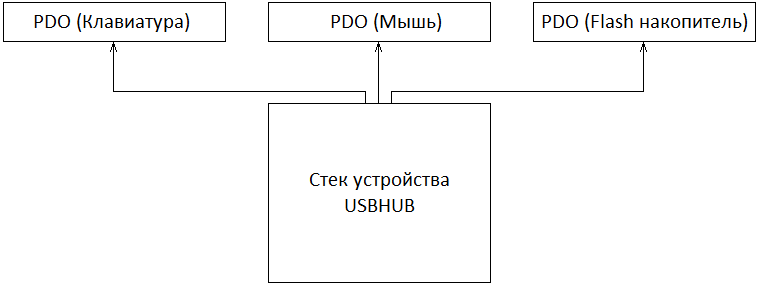
\includegraphics[width = \textwidth]{images/1.png}}
  \caption{}
\end{figure}

\par Как отражено на рисунке, в данном примере в качестве шины выступает драйвер USB-хаба. Конкретные DEVICE\_OBJECT стека устройства этого хаба не изображены для краткости и с целью сохранения последовательности пояснений.\\

\par Как только PnP менеджер получит список всех PDO, он по отдельности соберет всю необходимую информацию об этих устройствах. Например, будет послан запрос с minor кодом IRP\_MN\_QUERY\_ID. Посредством этого запроса PnP менеджер получит идентификаторы устройства, как аппаратные, так и совместимые. Также PnP менеджер соберет всю необходимую информацию о требуемых аппаратных ресурсах самим устройством. И так далее.\\

\par После того, как вся необходимая информация будет собрана, PnP менеджер создаст так называемую DevNode, которая будет отражать состояние устройства. Также PnP создаст ветку реестра для конкретного экземпляра устройства или откроет существующую, если устройство ранее подключалось к ПК.\\

\par Следующая задача PnP — это запуск драйвера устройства. Если драйвер не был ранее установлен, тогда PnP будет ожидать установки. Иначе, при необходимости, PnP загрузит его и передаст ему управление. Ранее упоминалось, что поле DriverExtension->AddDevice структуры DRIVER\_OBJECT содержит адрес обработчика, который вызывается всякий раз, когда система обнаруживает новое устройство. Прототип этого обработчика изображен ниже.\\

\begin{lstlisting}[language=c caption={Обработчик добавления устройства}]
NTSTATUS DispatchAddDevice( 
	PDRIVER_OBJECT DriverObject, 
	PDEVICE_OBJECT PhysicalDeviceObject 
); 
\end{lstlisting}

Всякий раз, когда PnP обнаруживает устройство, управлением которого занимается тот или иной драйвер, вызывается зарегистрированный обработчик этого драйвера, где ему передается указатель на PDO. Информация об установленном драйвере также хранится в соответствующей ветке реестра.\\

\par В задачу обработчика входит создание DEVICE\_OBJECT и его прикрепление к PDO. Прикрепленный DEVICE\_OBJECT также называют Functional Device Object или FDO. Именно этот FDO и будет отвечать за работу устройства и представление его интерфейсов в системе. Ниже представлен пример, когда PnP завершил вызов драйвера, отвечающего за работу устройства. \\


\begin{figure}[H]
  \centering
  \fbox{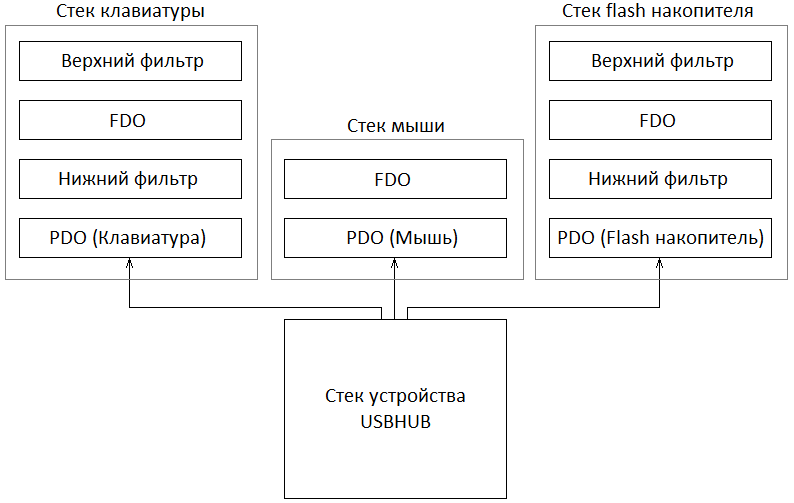
\includegraphics[width = \textwidth]{images/2.png}}
  \caption{}
\end{figure}

\par Как отражено на примере, кроме драйвера самого устройства также могут быть зарегистрированы нижние и верхние фильтры класса устройства. Следовательно, если таковые имеются, PnP также загрузит их драйвера и вызовет их AddDevice обработчики. Т.е. порядок вызова драйверов следующий: сначала загружаются и вызываются зарегистрированные нижние фильтры, затем загружается и вызывается драйвер самого устройства, и в завершении загружаются и вызываются верхние фильтры. Нижние и верхние фильтры являются обычным DEVICE\_OBJECT, которые создают драйвера и прикрепляют их к PDO в своих обработчиках AddDevice. Количество нижних и верхних фильтров не ограничено.\\

\par В этот момент стеки устройств полностью сформированы и готовы к работе. Поэтому PnP посылает запрос с minor кодом IRP\_MN\_START\_DEVICE. В ответ на этот запрос все драйвера стека устройства должны подготовить устройство к работе. И если в этом процессе не возникло проблем, тогда запрос завершается успешно. В противном случае, если любой из драйверов не может запустить устройство, тогда он завершает запрос с ошибкой. Следовательно, устройство не будет запущено.\\

\par Также, когда драйвер шины определяет, что произошли изменения на шине, он посредством функции IoInvalidateDeviceRelations уведомляет PnP о том, что следует заново собрать информацию о подключенных устройствах. В этот момент драйвер не удаляет ранее созданный PDO. Просто при получении запроса с minor кодом IRP\_MN\_QUERY\_DEVICE\_RELATIONS он не включит этот PDO в список. Затем PnP на основании полученного списка опознает новые устройства и устройства, которые были отключены от шины. PDO отключенных устройств драйвер удалит тогда, когда PnP пошлет запрос с minor кодом IRP\_MN\_REMOVE\_DEVICE. Для драйвера этот запрос означает, что устройство более никем не используется, и оно может быть безопасно удалено.\\

\subsection{Решение}

Суть самого решения заключается в создании верхнего фильтра класса USB-шины. Нас интересует класс USB с GUID равным 36fc9e60-c465-11cf-8056-444553540000. Как гласит MSDN, этот класс используется для USB хост контроллеров и хабов. Однако практически это не так, этот же класс используется flash-накопителями. Поэтому далее необходимо отсеять остальные устройства и блокировать только flash-накопители.

Код обработчика AddDevice представлен ниже.

\begin{lstlisting}[language=c caption={AddDevice обработчик}]
NTSTATUS UsbCreateAndAttachFilter( 
	PDEVICE_OBJECT PhysicalDeviceObject, 
	bool UpperFilter 
) {

	SUSBDevice*		USBDevice;
	PDEVICE_OBJECT		USBDeviceObject = nullptr;

	ULONG			Flags;

	NTSTATUS		Status = STATUS_SUCCESS;

	PAGED_CODE();

	for ( ;; ) {

		// если нижний фильтр уже прикреплен, тогда здесь больше делать нечего
		if ( !UpperFilter ) {
			USBDeviceObject = PhysicalDeviceObject;
			while ( USBDeviceObject->AttachedDevice ) {
				if ( USBDeviceObject->DriverObject == g_DriverObject ) {
					return STATUS_SUCCESS;
				}
				USBDeviceObject = USBDeviceObject->AttachedDevice;
			}
		}

		// создаем фильтр
		Status = IoCreateDevice(
			g_DriverObject,
			sizeof( SUSBDevice ),
			nullptr,
			PhysicalDeviceObject->DeviceType,
			PhysicalDeviceObject->Characteristics,
			false,
			&USBDeviceObject
		);
		if ( !NT_SUCCESS( Status ) ) {
			break;
		}

		// инициализируем флаги созданного устройства, копируем их из объекта к 
		// которому прикрепились
		Flags = PhysicalDeviceObject->Flags & 
		 (DO_BUFFERED_IO | DO_DIRECT_IO | DO_POWER_PAGABLE);
		USBDeviceObject->Flags |= Flags;

		// получаем указатель на нашу структуру
		USBDevice = (SUSBDevice*)USBDeviceObject->DeviceExtension;

		// инициализируем деструктор
		USBDevice->DeleteDevice = DetachAndDeleteDevice;

		// инициализируем обработчики
		for ( ULONG i = 0; i <= IRP_MJ_MAXIMUM_FUNCTION; i++ ) {
			USBDevice->MajorFunction[i] = UsbDispatchCommon;
		}
		USBDevice->MajorFunction[IRP_MJ_PNP] = UsbDispatchPnp;
		USBDevice->MajorFunction[IRP_MJ_POWER] = UsbDispatchPower;

		// инициализируем семафор удаления устройства
		IoInitializeRemoveLock( 
			&USBDevice->Lock, 
			USBDEVICE_REMOVE_LOCK_TAG, 
			0, 
			0 
		);

		// заполняем структуру
		USBDevice->SelfDevice = USBDeviceObject;
		USBDevice->BaseDevice = PhysicalDeviceObject;
		USBDevice->UpperFilter = UpperFilter;

		// инициализируем paging семафор
		USBDevice->PagingCount = 0;
		KeInitializeEvent( &USBDevice->PagingLock, SynchronizationEvent, true );

		// прикрепляем устройство к PDO
		USBDevice->LowerDevice = IoAttachDeviceToDeviceStack( 
			USBDeviceObject, 
			PhysicalDeviceObject 
		);
		if ( !USBDevice->LowerDevice ) {
			Status = STATUS_NO_SUCH_DEVICE;
			break;
		}

		break;

	}

	// в зависимости от результата делаем

	if ( !NT_SUCCESS( Status ) ) {

		// отчистку

		if ( USBDeviceObject ) {
			IoDeleteDevice( USBDeviceObject );
		}

	} else {

		// или сбрасываем флаг инициализации
		USBDeviceObject->Flags &= ~DO_DEVICE_INITIALIZING;

	}

	return Status;

}

static NTSTATUS DispatchAddDevice( 
	PDRIVER_OBJECT DriverObject, 
	PDEVICE_OBJECT PhysicalDeviceObject 
) {

	UNREFERENCED_PARAMETER( DriverObject );

	return UsbCreateAndAttachFilter( PhysicalDeviceObject, true );

}
\end{lstlisting}

Здесь создается DEVICE\_OBJECT и прикрепляется его к PDO. Таким образом, будут перехватываться все запросы, направленные к USB-шине. \\

\par В нашу задачу входит перехватывать запросы с minor кодом IRP\_MN\_START\_DEVICE. Код обработчика этого запроса изображен ниже.

\begin{lstlisting}[language=c caption={Перехват сигнала о запуске работы устройства}]
static NTSTATUS UsbDispatchPnpStartDevice( SUSBDevice* USBDevice, PIRP Irp ) {

	bool		HubOrComposite;
	NTSTATUS	Status;

	PAGED_CODE();

	for ( ;; ) {

		// проверить, позволено ли устройству работать, также обновить
		// информацию об устройстве, является ли оно хабом или композитным
		Status = UsbIsDeviceAllowedToWork( &HubOrComposite, USBDevice );
		if ( !NT_SUCCESS( Status ) ) {
			break;
		}
		USBDevice->HubOrComposite = HubOrComposite;

		// продвинуть запрос
		Status = ForwardIrpSynchronously( USBDevice->LowerDevice, Irp );
		if ( !NT_SUCCESS( Status ) ) {
			break;
		}

		break;

	}

	// завершаем запрос
	Irp->IoStatus.Status = Status;
	IoCompleteRequest( Irp, IO_NO_INCREMENT );

	// и освобождаем устройство
	IoReleaseRemoveLock( &USBDevice->Lock, Irp );

	return Status;

}
\end{lstlisting}

Как изображено на рисунке, обработчик вызывает функцию UsbIsDeviceAllowedToWork. Эта функция выполняет все необходимые проверки, чтобы определить, разрешено ли устройству работать. В первую очередь функция позволяет всегда работать хабам и композитным устройствам, клавиатурам и мышам. А также тем устройствам, которые находятся в списке разрешенных. Если функция возвращает неуспешный код возврата, тогда запрос завершается с ошибкой. Таким образом, работа устройства будет заблокирована. \\

\par Функция определяет, является ли устройство хабом или композитным устройством. Это необходимо потому, что, как уже было упомянуто, класс устройств, который используется для flash накопителей, используется не только этими устройствами. Т.е. для хабов и композитных устройств дополнительно перехватывается запрос перечисления дочерних устройств, на этом этапе, важно также прикрепить ко всем дочерним устройствам фильтр, и этот фильтр будет нижним. В противном случае контроль над дочерними устройствами будет потерян.\\

\par Все упомянутые определения выполняются на основе идентификаторов устройств. \\

\par Для загрузки драйвера на 64 битной версии Windows требуется цифровая подпись, иначе служба безопасности не даст его запустить: 

\begin{figure}[H]
  \centering
  \fbox{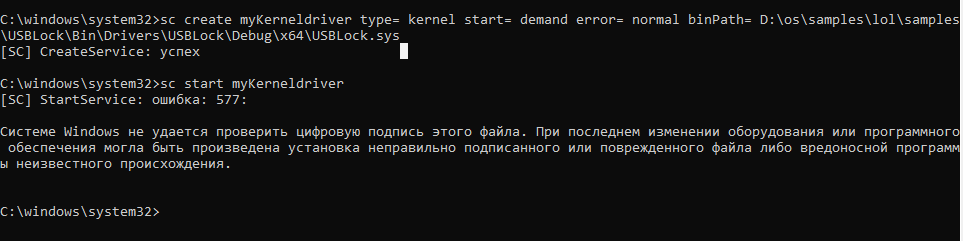
\includegraphics[width = \textwidth]{images/3.png}}
  \caption{}
\end{figure}

Цифровая подпись является электронной меткой безопасности, которая может указать издателя данного программного обеспечения, а также факт изменения драйвера после его подписания. Если драйвер подписан издателем и достоверность подписи подтверждена центром сертификации, то можно быть уверенным, что драйвер выпущен именно этим издателем и не подвергался изменениям.

\section{Вывод}
    В ходе выполнения курсовой работы был написан драйвер уровня ядра для блокирования подключения устройств flash-накопителей. Но при этом другие usb устройства могут свободно работать. Для реализации данной функциональности был написан драйвер фильтр, который перехватывает запрос на запуск устройства и проверяет является ли он flash накопителем. Для полноценного использования драйвера необходимо обойти проверку цифровой подписи или создать ее для данного драйвера.
\end{document}